\chapter{Технологический раздел}

\section{Выбор языка программирования}
Для создания программного комплекса был выбран язык программирования C++. Этот выбор был сделан на основании того, что данный язык позволяет делать всё то, что необходимо в рамках этой работы, а именно: создание и управвление потоками, соединение и передача данных по сокетам, блокировка на мьютексах, работа с контейнерами.

\section{Выбор протокола транспортного уровня}
Взаимодействие между сервером и клиентами должно осуществляться на основании собственного протокола, основанного на протоколе TCP. Данный протокол выбран в связи с тем, что потеря данных между клиентами - недопустима. Протокол TCP (Transmission Control Protocol — протокол управления передачей) был специально разработан для обеспечения надежного сквозного байтового потока по ненадежной интерсети. \cite{tanenbaum-comp-networks}

\section{Проблемы многопоточности}
При работе сервера приложения несколько потоков работают с одними и теми же данными. Для взаимоисключений используются мьютексы.

Мьютекс (mutex) - это фактически блокировка, которая устанавливается (запирается) перед обращением к разделяемому ресурсу и
снимается (отпирается) после выполнения требуемой последовательности операций. Если мьютекс заперт, то любой другой поток, который попытается запереть его, будет заблокирован до тех пор, пока мьютекс не будет отперт. Если в момент, когда отпирается мьютекс, заблокированными окажутся несколько потоков, все они будут запущены и первый из них, который успеет запереть мьютекс, продолжит работу. Все остальные потоки обнаружат, что мьютекс по-прежнему заперт, и опять перейдут в режим ожидания. Таким образом, доступ к ресурсу сможет получить одновременно только один поток. \cite{rago-unix}

\section{Используемые шаблоны проектирования}

При реализации программного комплекса использовались шаблоны проектирования singlton и шаблонный метод.  \cite{gof}

\subsection{Паттерн singleton}

Класс сервера игры основан на паттерне singleton. Это обосновывается тем, что в одной программе больше одного объекта сервера создавать не имеет смысла.

\lstinputlisting[language=C++, caption={Header файл.}]{code/singleton.h}

\lstinputlisting[language=C++, caption={Реализация.}]{code/singleton.cpp}


\subsection{Паттерн шаблонный метод}

Необходимо написать класс клиента игры и сделать его абстрактным. В этом классе реализуем методы, нужные для общения с сервером (обмен сообщениями о начале и конце игры). В этом классе будет чисто абстрактная функция, которая сделает класс абстрактным. Этот метод нужно реализовать в классе наследнике, он будет реализовывать обмен сообщениями конкретной игры.

В ~\ref{listing:ClientGameTwoPlayers} создаем абстрактный класс. 

В ~\ref{listing:ClientPinball} создаем класс ClientPinball и наследуем его от класса ClientGameTwoPlayers. Реализуем абстрактную функцию из родительского класса, которая будет отвечать за передачу сообщений и данных, специфичные для данной игры.

\lstinputlisting[language=C++, caption={Header файл для родительского класса}, label=listing:ClientGameTwoPlayers]{code/template_method.h}

\lstinputlisting[language=C++, caption={Реализация для класса потомка}, label=listing:ClientPinball]{code/template_method.cpp}

\section{Примеры кода}

\begin{lstlisting}[language=C++, caption={Создание соединения с сервером на клиенте},label=DescriptiveLabel]
bool ClientGameTwoPlayers::initConnection(char *ipServer, int portServer) {
  mutexArrBalls = PTHREAD_MUTEX_INITIALIZER;
  mutexNewBall = PTHREAD_MUTEX_INITIALIZER;
  mutexFlipper = PTHREAD_MUTEX_INITIALIZER;

  if (this->getState() != STATE_CLIENT::CREATE) {
    return false;
  }

  sock = socket(AF_INET, SOCK_STREAM, 0);
  if (sock < 0) {
    perror("socket");
    return false;
  }

  addr.sin_family = AF_INET;
  addr.sin_port = htons(portServer);
  addr.sin_addr.s_addr = inet_addr(ipServer);

  if (connect(sock, (struct sockaddr *) &addr, sizeof (addr)) < 0) {
    perror("connect");
    return false;
  }

  this->setState(STATE_CLIENT::CONNECT);
  return true;
}
\end{lstlisting}

\begin{lstlisting}[language=C++, caption={Подготовка сервера к слушанию клиентов},label=DescriptiveLabel]
bool ServerPinball::initConnection(int port) {
  w_lock = PTHREAD_MUTEX_INITIALIZER;
  p_lock = PTHREAD_MUTEX_INITIALIZER;

  struct sockaddr_in addr;

  listener = socket(AF_INET, SOCK_STREAM, 0);
  if (listener < 0) {
    perror("socket");
    return false;
  }
  addr.sin_family = AF_INET;
  addr.sin_port = htons(port);
  addr.sin_addr.s_addr = htonl(INADDR_ANY);
  if (bind(listener, (struct sockaddr *) &addr, sizeof (addr)) < 0) {
    perror("bind");
    return false;
  }

  this->setPort(port);
  listen(listener, MAX_COUNT_PAIR_PLAYERS * 2 + MAX_LENGTH_QUEUE_WAITING_PLAYERS);
  logger->printlog("server is created");
  printf("server is created\n");
  return true;
}
\end{lstlisting}

\begin{lstlisting}[language=C++, caption={Структуры данных передаваемых пакетов},label=DescriptiveLabel]
typedef struct {
  float x;
  float y;
  float rotation;
} SimpleBall;

typedef struct {
  float x;
  float y;
  float speedX;
  float speedY;
  float rotation;
} PhysicsBall;

typedef struct {
  bool left;
  bool right;
  float spring;
  int score;
} FlipperTriggered;

\end{lstlisting}

\begin{lstlisting}[language=C++, caption={Отправка/прием типа сообщения},label=DescriptiveLabel]
static void sendTypeMessage(int sock, TYPE_OF_MSG code) {
  send(sock, &code, sizeof (code), 0);
}

static TYPE_OF_MSG receiveTypeMessage(int sock) {
  TYPE_OF_MSG code;
  recv(sock, &code, sizeof (code), 0);
  return code;
}
\end{lstlisting}

\begin{lstlisting}[language=C++, caption={Отправка/прием сообщения о старте игры},label=DescriptiveLabel]
static void sendStartGame(PairPlayers* pair) {
  TYPE_OF_MSG code = TYPE_OF_MSG::START;
  sendTypeMessage(pair->playerOne, code);
  sendTypeMessage(pair->playerTwo, code);
}

static bool receiveStartGame(PairPlayers* pair) {
  TYPE_OF_MSG code = receiveTypeMessage(pair->playerOne);
  if (code != TYPE_OF_MSG::START)
    return false;

  return receiveTypeMessage(pair->playerTwo) == TYPE_OF_MSG::START;
}

\end{lstlisting}

\begin{lstlisting}[language=C++, caption={Отправка/прием сообщения с именем},label=DescriptiveLabel]
static bool receiveNamePlayers(PairPlayers* pair, char namePlayer1[MAX_LENGTH_NAME_PLAYER], char namePlayer2[MAX_LENGTH_NAME_PLAYER]) {
  sendTypeMessage(pair->playerOne, TYPE_OF_MSG::RECEIVE_NAME);
  recv(pair->playerOne, namePlayer1, MAX_LENGTH_NAME_PLAYER * sizeof (char), 0);

  sendTypeMessage(pair->playerTwo, TYPE_OF_MSG::RECEIVE_NAME);
  recv(pair->playerTwo, namePlayer2, MAX_LENGTH_NAME_PLAYER * sizeof (char), 0);

  return true;
}

static void sendNamePlayers(PairPlayers* pair, char namePlayer1[MAX_LENGTH_NAME_PLAYER], char namePlayer2[MAX_LENGTH_NAME_PLAYER]) {
  sendTypeMessage(pair->playerOne, TYPE_OF_MSG::SEND_NAME);
  send(pair->playerOne, namePlayer2, MAX_LENGTH_NAME_PLAYER * sizeof (char), 0);

  sendTypeMessage(pair->playerTwo, TYPE_OF_MSG::SEND_NAME);
  send(pair->playerTwo, namePlayer1, MAX_LENGTH_NAME_PLAYER * sizeof (char), 0);
}
\end{lstlisting}

\begin{lstlisting}[language=C++, caption={Отправка массива шаров},label=DescriptiveLabel]
void ClientGameTwoPlayers::sendArrBalls(int count, SimpleBall arr[MAX_COUNT_BALLS]) {
  sendTypeMessage(sock, TYPE_OF_MSG::ARR_BALL);
  send(sock, &count, sizeof (int), 0);
  send(sock, arr, count * sizeof (SimpleBall), 0);
}
\end{lstlisting}

\begin{lstlisting}[language=C++, caption={Отправка информации о рычаге, пружине, счете},label=DescriptiveLabel]
void ClientGameTwoPlayers::sendFlipperTriggered(FlipperTriggered &flipperTriggered) {
  sendTypeMessage(sock, TYPE_OF_MSG::FLIPPER_TRIGGERED);
  send(sock, &flipperTriggered, sizeof (flipperTriggered), 0);
}
\end{lstlisting}

\begin{lstlisting}[language=C++, caption={Получение данных типа Т},label=DescriptiveLabel]
virtual void toListenServerData(TYPE_OF_MSG code) {
  if (code == TYPE_OF_MSG::FLIPPER_TRIGGERED) {
    FlipperTriggered *flipperTriggered = new FlipperTriggered;
    mutexFlipperLock();
    recv(sock, flipperTriggered, sizeof (FlipperTriggered), 0);
    queueFlipperTriggered.push(flipperTriggered);
    mutexFlipperUnlock();
  } else if (code == TYPE_OF_MSG::ARR_BALL) {
    ArrayBalls *arrayBalls = new ArrayBalls;
    mutexArrBallsLock();
    recv(sock, &(arrayBalls->countSimpleBalls), sizeof (arrayBalls->countSimpleBalls), 0);
    recv(sock, arrayBalls->arrBallsOpponent, arrayBalls->countSimpleBalls * sizeof (SimpleBall), 0);
    queueArrBallsOpponent.push(arrayBalls);
    mutexArrBallsUnlock();
  } else if (code == TYPE_OF_MSG::NEW_BALL) {
    PhysicsBall *physicsBall = new PhysicsBall;
    mutexNewBallLock();
    recv(sock, physicsBall, sizeof (PhysicsBall), 0);
    queueNewBall.push(physicsBall);
    mutexNewBallUnlock();
  } 
}
\end{lstlisting}

\section{Интерфейс взаимодействия с клиентом}

Интерфейс взаимодействия с клиентом представлен следующими функциями:
\begin{lstlisting}[language=C++, caption={Интерфейс взаимодействия с клиентом},label=DescriptiveLabel]
  ClientGameTwoPlayers();
  ~ClientGameTwoPlayers();
  bool createConnection(char *ipServer);
  bool createConnection(char *ipServer, int portServer);
  bool handshake(char name[MAX_LENGTH_NAME_PLAYER]);
  bool launchServesServer();
  STATE_CLIENT getState();
  void setFinish();
  char *getMyName();
  char *getOpponentName();

  bool getNewBall(PhysicsBall &ball);
  bool getArrBallsOpponent(SimpleBall arr[MAX_COUNT_BALLS], int &count);
  bool getFlipperTriggered(FlipperTriggered &flipper);

  void sendArrBalls(int count, SimpleBall arr[MAX_COUNT_BALLS]);
  void sendNewBall(PhysicsBall &newBall);
  void sendFlipperTriggered(FlipperTriggered &flipperTriggered);
  
  void clearArrBalls(int countOpp);
\end{lstlisting}

\section{Логгер сервера}

\lstinputlisting[language=C++, caption=Логгер]{code/logger.h}

\begin{figure}[h]
  \centering
  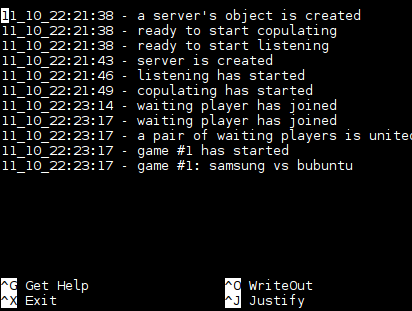
\includegraphics[scale=1.5]{log.png}
  \caption{Пример логга.}
  \label{image:servermenu}
\end{figure}

\section{Инструкция по компиляции и запуску игры}

Исходные тексты игры можете скачать из данного репозитория \href{https://github.com/iproha94/MultiplayerPinball}{https://github.com/iproha94/MultiplayerPinball}.

\begin{enumerate}
\item Установите Ubuntu. 

(c Debian могут возникнуть проблемы при запуске скрипта install-deps-linux.sh, пишет что проблемы с OpenGL)

\item Скачайте cocos2d-x-3.6 

(именно эта версия должна быть, более новые версия искажают физическое пространство для данной игры) 

\item зайдите в папку с распакованным cocos2d 
\item  ./build/install-deps-linux.sh
\item  ./tools/travis-scripts/install\_glfw.sh
\item  ./setup.py
\item  mkdir build/linux-build 
\item  cd build/linux-build 
\item  cmake ../.. 
\item  make 

(на данном этапе будут выскакивать ошибки, связанные с isnan, в файлах, в которых происходят эти ошибки перед isnan надо написать "std::" без кавычек) 

\item  ./bin/cpp-tests/cpp-tests 

\item  Возвращаемя в основную папку кокоса. Создание нового проекта:

cocos new MyGame -p com.your\_company.mygame -l cpp -d NEW\_PROJECTS\_DIR 

\item  Запуск 

cocos run -s NEW\_PROJECTS\_DIR/MyGame -p linux 

\item В NEW\_PROJECTS\_DIR/MyGame удалите папку Classes, Resources и файл CMakeLists.txt 
\item Склонируйте данный репозиторий 
\item Переместите папки Classes, Resources и файл CMakeLists.txt в папку NEW\_PROJECTS\_DIR/MyGame 
\item Из папки Multiplayer переместите файлы, в которых нет слова "server" в папку Classes
\end{enumerate}

\section{Запуск сервера}

Компиляция исходных кодов сервера осуществляется командами \ref{CompilationServer}

\begin{lstlisting}[language=bash, caption={Компиляция исходных кодов сервера},label=CompilationServer]
g++ -c -std=c++11 mainServerPinball.cpp serverPinball.cpp 
g++ -pthread -std=c++11 mainServerPinball.o serverPinball.o -o serexe
\end{lstlisting}

Программа сервера не написана в виде демона. При развертывании программы удобно будет использовать утилиту screen. Screen создает отдельные объекты, называемые иногда «скринами». Каждый скрин - это что-то вроде окна, которое можно свернуть-развернуть, если проводить аналогию с графическим интрефейсом. Только вместо окна вы получаете виртуальную консоль, которую можно отправить в фон или вывести на передний план, и в которой запускается указанное приложение.

\section{Интерфейс взаимодействия сервера с пользователем}

Интерфейс взаимодействия сервера с пользователем представлен дружественным консольным меню ~\ref{image:servermenu} 

В меню отображается следующая информация:
\begin{enumerate}
\item launched - создан ли серверный сокет
\item listening - прослушиваются ли входящие соединения 
\item copulation - соединяются ли в пары подсоединяющиеся игроки
\item port - номер порта сервера
\item quantity of waiteng players - количество ожидающих соединения игроков
\item quantity of pair of players - количество сессий (играющих пар игроков)
\item full quantity of games - количество сыгранных игр
\end{enumerate}

Управление сервером осущестляется следующими командами:
\begin{enumerate}
\item 1 - создать соединение с стандартным портом (49876)
\item 2 - создать соединение с портом, которое нужно будет ввести с клавиатуры
\item 3 - закрыть соединение
\item 4 - начать слушать входящие соединения
\item 5 - перестать слушать входящие соединения
\item 6 - начать соединять в пары ожидающих игроков
\item 7 - перестать соединять в пары ожидающих игроков
\item 8 - обновить информацию о состоянии сервера
\item 0 - выход из программы
\end{enumerate}

\begin{figure}[h]
  \centering
  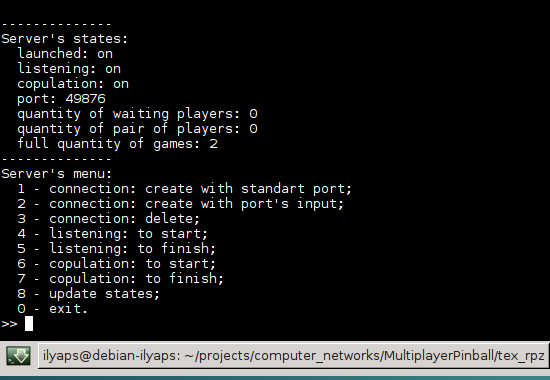
\includegraphics{servermenu.png}
  \caption{Меню сервера.}
  \label{image:servermenu}
\end{figure}

